\documentclass{article}

% if you need to pass options to natbib, use, e.g.:
%     \PassOptionsToPackage{numbers, compress}{natbib}
% before loading neurips_2018

% ready for submission
% \usepackage{neurips_2018}

% to compile a preprint version, e.g., for submission to arXiv, add add the
% [preprint] option:
%     \usepackage[preprint]{neurips_2018}

% to compile a camera-ready version, add the [final] option, e.g.:
     \usepackage[final]{nips_2018}

% to avoid loading the natbib package, add option nonatbib:
%     \usepackage[nonatbib]{neurips_2018}

\usepackage[utf8]{inputenc} % allow utf-8 input
\usepackage[T1]{fontenc}    % use 8-bit T1 fonts
\usepackage{hyperref}       % hyperlinks
\usepackage{url}            % simple URL typesetting
\usepackage{booktabs}       % professional-quality tables
\usepackage{amsfonts}       % blackboard math symbols
\usepackage{nicefrac}       % compact symbols for 1/2, etc.
\usepackage{microtype}      % microtypography

\usepackage{amsmath}
\usepackage{amsfonts}
\usepackage{amssymb}
\usepackage{amsthm}
\usepackage{mathrsfs}
\usepackage{graphicx}
	\graphicspath{{./image/}}

\title{\emph{MATH6450E Project 1:} Latent Dirichlet Allocation using Variational Inference}

% The \author macro works with any number of authors. There are two commands
% used to separate the names and addresses of multiple authors: \And and \AND.
%
% Using \And between authors leaves it to LaTeX to determine where to break the
% lines. Using \AND forces a line break at that point. So, if LaTeX puts 3 of 4
% authors names on the first line, and the last on the second line, try using
% \AND instead of \And before the third author name.

\author{%
  FAN Min
  \thanks{\url{https://github.com/ProteusFAN/MATH6450E/tree/master/Latent\%20Dirichlet\%20Allocation\%20using\%20Variational\%20Inference}} \\
  Department of Mathematics\\
  Hong Kong University of Science and Technology\\
  \texttt{mfanab@connect.ust.hk} \\
  % examples of more authors
  % \And
  % Coauthor \\
  % Affiliation \\
  % Address \\
  % \texttt{email} \\
  % \AND
  % Coauthor \\
  % Affiliation \\
  % Address \\
  % \texttt{email} \\
  % \And
  % Coauthor \\
  % Affiliation \\
  % Address \\
  % \texttt{email} \\
  % \And
  % Coauthor \\
  % Affiliation \\
  % Address \\
  % \texttt{email} \\
}

\begin{document}
% \nipsfinalcopy is no longer used

\maketitle

\begin{abstract}
   Latent Dirichlet allocation (LDA) is a famous topic modeling algorithm proposed at the beginning of the $ 21^{\mathrm{th}} $ century, which is a three-level hierarchical Bayesian model. Variational inference is implemented in E-step of EM algorithm to approximate the posterior distribution of the latent variables. Under the framework of EM algorithm, the log-likelihood of observed variables is maximized and meanwhile the parameters in the model are learned from training data. In this report, we deduced LDA algorithm and did simulation on a small corpus. 
\end{abstract}

\section{Introduction}

Latent Dirichlet allocation (LDA) is a three-level hierarchical generative probabilistic model, which generates text as \ref{figure_lda} shows. $ N $ is the number of the documents. $ N_{i} $ is the number of words in document $ i $, which follows Poisson distribution in generating process . $ K $ is the number of topics. $ M $ is the number of words in vocabulary. $ \theta_{i} $ is a $ K $-length vector as the parameter of Multinomial distribution. $ \alpha $ is a $ K $-length vector as the parameter of Dirichlet distribution as the prior of $ \theta_{i} $. $ \varphi_{k} $ is a $ M $-length vector as the parameter of Multinomial distribution. $ \beta $ is a $ M $-length vector as the parameter of Dirichlet distribution as the prior of $ \varphi_{k} $. $ z_{i,j} $ refers to topic index in topic list of word $ j $ in document $ i $. $ w_{i,j} $ refers to the word index in vocabulary of word $ j $ in document $ i $.

\begin{figure}[htbp]
	\centering
	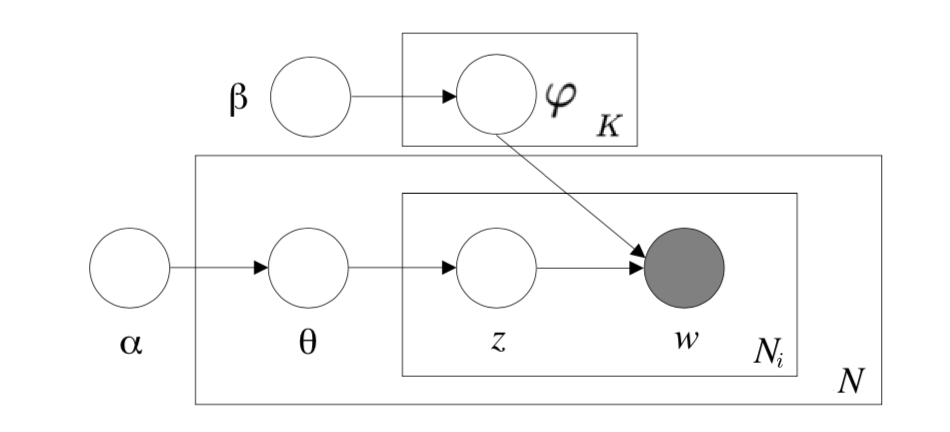
\includegraphics[width = 0.7\linewidth]{lda}
	\caption{Latent Dirichlet Allocation}
	\label{figure_lda}
\end{figure}

\section{Method}

The goal is to maximize the log-likelihood of observed variables with respect to parameter $ \alpha $ and $ \varphi $, that is,
\begin{align*}
	p(w | \alpha, \varphi) &= \int p(\theta | \alpha) (\prod^{N_i}_{n=1} \sum^{K}_{k=1} p(z_n=k | \theta) p(w_n | z_n=k)) d\theta \\
	&= \int p(\theta | \alpha)(\prod^{N_i}_{n=1} \sum^{K}_{k=1} \prod^M_{j=1}(\theta_k \varphi_{kj})^{w_n^{j}}) d\theta,
\end{align*}
which is not analytically tractable. EM algorithm is to maximize the log-likelihood of the observed variables.

\subsection{E-step}
The posterior distribution of latent variables
\begin{equation*}
	p(\theta, z | w, \alpha, \varphi) = \frac{p(\theta, z, w | \alpha, \varphi)}{p(w | \alpha, \varphi)}
\end{equation*}
is hard to compute. Mean-field variational inference is implemented to approximate $ p(\theta, z | w, \alpha, \varphi) $ by $ q(\theta, z | \gamma, \phi) $, where
\begin{equation*}
	q(\theta, z | \gamma, \phi) = q(\theta | \gamma) \prod^{N_i}_{n=1} q(z_n | \phi_n).
\end{equation*}

\begin{figure}[htbp]
	\centering
	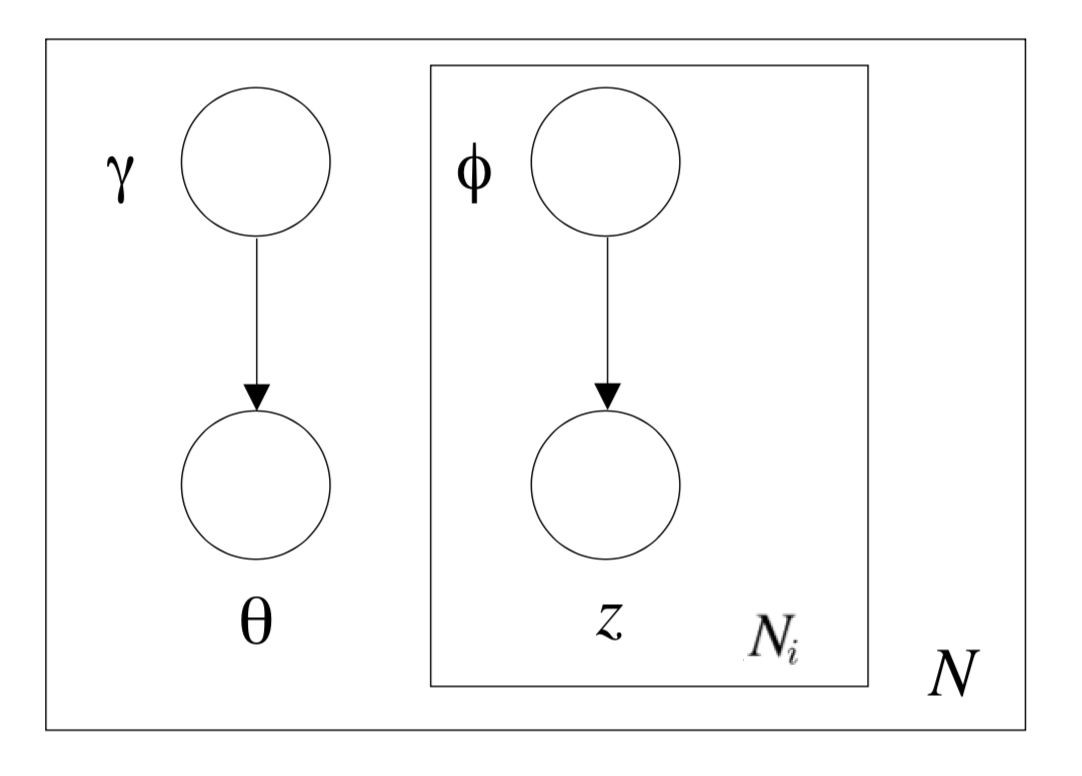
\includegraphics[width = 0.4\linewidth]{vi}
	\caption{Mean-field variational approximation}
	\label{figure_vi}
\end{figure}

The difference between two distributions is measured by KL-divergence. So the solution is given by
\begin{equation*}
	(\gamma^{\ast}, \phi^{\ast}) = \mathrm{argmin}_{\gamma,\phi} KL(q(\theta, z | \gamma, \phi) || p(\theta, z|w, \alpha, \varphi)).
\end{equation*}
It is easy to show
\begin{equation*}
	\log(p(w | \alpha, \varphi)) = \mathcal{L}(\gamma, \phi; \alpha, \varphi) + KL(q(\theta, z | \gamma, \phi) || p(\theta, z|w, \alpha, \varphi),
\end{equation*}
where
\begin{equation*}
	\mathcal{L}( \gamma, \phi; \alpha, \varphi) = E_q[\log(p(\theta, z, w | \alpha, \varphi))] - E_q[\log(q(\theta, z | \gamma, \phi))].
\end{equation*}
So minimizing $ KL(q(\theta, z | \gamma, \phi) || p(\theta, z|w, \alpha, \varphi) $ is equivalent to maximizing $ \mathcal{L}( \gamma, \phi; \alpha, \varphi) $.
\vspace{1em}

\subsubsection{Computing $ \mathcal{L}( \gamma, \phi; \alpha, \varphi) $}
It is easy to show
\begin{align*}
	\mathcal{L}( \gamma, \phi; \alpha, \varphi) &= E_q[\log(p(\theta, z, w | \alpha, \varphi))] - E_q[\log(q(\theta, z | \gamma, \phi))] \\
	&= E_q[\log(p(\theta | \alpha))] + E_q[\log(p(z | \theta))] + E_q[\log(p(w | z, \varphi))] \\
	&\quad - E_q[\log(q(\theta | \gamma))] - E_q[\log(q(z | \phi))].
\end{align*}
In order to compute $ \mathcal{L}( \gamma, \phi; \alpha, \varphi) $, we just need to compute these five terms.
\vspace{1em}

As for the first term $ E_q[\log(p(\theta | \alpha))] $,
\begin{align*}
	E_q[\log(p(\theta | \alpha))] &= \sum^{K}_{i=1}(\alpha_i - 1) E_q[\log \theta_i] + \log \Gamma(\sum^{K}_{i=1} \alpha_i) - \sum^{K}_{i=1}\log \Gamma(\alpha_i)\\
	&= \sum^{K}_{i=1}(\alpha_i - 1)(\psi(\gamma_i) - \psi(\sum^{K}_{j=1} \gamma_j)) + \log \Gamma(\sum^{K}_{i=1} \alpha_i) - \sum^{K}_{i=1}\log \Gamma(\alpha_i),
\end{align*}
where $ \theta $ is generated from $ Dir(\theta|\gamma) $ and $ \psi $ is digamma function.

As for the second term $ E_q[\log(p(z | \theta))] $,
\begin{align*}
	E_q[\log(p(z | \theta))] &= E_q[\sum^{N_d}_{n=1}\sum^{K}_{i=1}z_{ni}\log \theta_i] \\
	&= \sum^{N_d}_{n=1}\sum^{K}_{i=1}E_q[z_{ni}] E_q[\log\ theta_i] \\
	&= \sum^{N_d}_{n=1}\sum^{K}_{i=1} \phi_{ni}(\psi(\gamma_i) - \psi(\sum^{K}_{j=1}\gamma_j)),
\end{align*}
where $ z $ is generated from $ \mathrm{Multinomial}(z|\phi) $ and $ N_d $ is the number of words in document $ d $.

As for the third term $ E_q[\log(p(w | z, \varphi))] $,
\begin{align*}
	E_q[\log(p(w | z, \varphi))] &= E_q[\sum^{N_d}_{n=1}\sum^{K}_{i=1}\sum^{M}_{j=1} z_{ni} w^{j}_{n}\log\varphi_{ij}] \\
	&= \sum^{N_d}_{n=1}\sum^{K}_{i=1}\sum^{M}_{j=1}E_q[z_{ni}]w^{j}_{n}\log\varphi_{ij} \\
	&= \sum^{N_d}_{n=1}\sum^{K}_{i=1}\sum^{M}_{j=1}\phi_{ni}w^{j}_{n}\log\varphi_{ij}.
\end{align*}

As for the fourth term $ E_q[\log(q(\theta | \gamma))] $,
\begin{align*}
	E_q[\log(q(\theta | \gamma))] &= \sum^{K}_{i=1}(\gamma_i-1) E_q[\log\theta_i] + \log\Gamma(\sum^{K}_{i=1}\gamma_i) - \sum^{K}_{i=1}log\Gamma(\gamma_i) \\
	&= \sum^{K}_{i=1}(\gamma_i-1)(\psi(\gamma_i) - \psi(\sum^{K}_{j=1}\gamma_j)) + \log\Gamma(\sum^{K}_{i=1}\gamma_i) - \sum^{K}_{i=1}log\Gamma(\gamma_i).
\end{align*}

As for the fifth term $ E_q[\log(q(z|\phi))] $,
\begin{align*}
	E_q[\log(q(z | \phi))] &= E_q[\sum^{N_d}_{n=1}\sum^{K}_{i=1}z_{ni}\log\phi_{ni}] \\
	&= \sum^{N_d}_{n=1}\sum^{K}_{i=1}E_q[z_{ni}]\log\phi_{ni} \\
	&= \sum^{N_d}_{n=1}\sum^{K}_{i=1}\phi_{ni}\log\phi_{ni}.
\end{align*}

Finally, we have
\begin{align*}
\mathcal{L}( \gamma, \phi; \alpha, \varphi) &= \sum^{K}_{i=1}(\alpha_i - 1)(\psi(\gamma_i) - \psi(\sum^{K}_{j=1} \gamma_j)) + \log \Gamma(\sum^{K}_{i=1} \alpha_i) - \sum^{K}_{i=1}\log \Gamma(\alpha_i) \\
&\quad + \sum^{N_d}_{n=1}\sum^{K}_{i=1} \phi_{ni}(\psi(\gamma_i) - \psi(\sum^{K}_{j=1}\gamma_j)) \\
&\quad + \sum^{N_d}_{n=1}\sum^{K}_{i=1}\sum^{M}_{j=1}\phi_{ni}w^{j}_{n}\log\varphi_{ij} \\
&\quad - \sum^{K}_{i=1}(\gamma_i-1)(\psi(\gamma_i) - \psi(\sum^{K}_{j=1}\gamma_j)) + \log\Gamma(\sum^{K}_{i=1}\gamma_i) - \sum^{K}_{i=1}log\Gamma(\gamma_i) \\
&\quad - \sum^{N_d}_{n=1}\sum^{K}_{i=1}\phi_{ni}\log\phi_{ni} 
\end{align*}

\subsubsection{Updating $  \gamma, \phi $}
We update $ \phi $ first. Because $ \sum^{K}_{j=1}\phi_{ni} = 1 $, we implement Lagrange Multiplier and have
\begin{equation*}
	\mathcal{L}_{\phi_{ni}} = \phi_{ni}(\psi(\gamma_i) - \psi(\sum^{K}_{j=1}\gamma_j)) + \phi_{ni}\log\varphi_{iw} - \phi_{ni}\log\phi_{ni} + \lambda(\sum^{K}_{j=1}\phi_{ni}-1),
\end{equation*}
and take derivative
\begin{equation*}
	\frac{\partial{\mathcal{L}}}{\partial{\phi_{ni}}} = (\psi(\gamma_i)-\psi(\sum^{K}_{j=1}\gamma_j)) + \log\varphi_{iw} -\log\phi_{ni} - 1 + \lambda,
\end{equation*}
and let it be 0 whereby we have
\begin{equation*}
	\phi_{ni} \propto \varphi_{iw}\exp(\psi(\gamma_i) - \psi(\sum^{K}_{j=1}\gamma_j)).
\end{equation*}
We update $ \gamma $ next.
\begin{equation*}
	\mathcal{L}_{\gamma} = \sum^{K}_{i=1}(\psi(\gamma_i) - \psi(\sum^{K}_{j=1}\gamma_j))(\alpha_i + \sum^{N_d}_{n=1}\phi_{ni} - \gamma_{i}) - \log\Gamma(\sum^{K}_{i=1}\gamma_i) + \sum^{K}_{i=1}log\Gamma(\gamma_i)),
\end{equation*}
and take derivative
\begin{equation*}
	\frac{\partial{\mathcal{L}}}{\partial{\gamma_{i}}} = \psi{‘}(\gamma_i)(\alpha_i + \sum^{N_d}_{n=1}\phi_{ni} - \gamma_i) - \psi{‘’}(\sum^{K}_{j=1}\gamma_{j}) \sum^{K}_{j=1}(\alpha_j + \sum^{N_d}_{n=1}\phi_{nj} - \gamma_j),
\end{equation*}
and let it be 0 whereby we have
\begin{equation*}
	\gamma_i = \alpha_i + \sum^{N_d}_{n=1}\phi_{ni}.
\end{equation*}

We initialize $ \phi_{ni}^{0} $ to be $ \frac{1}{K} $ for all $ i, n $ and $ \gamma_i $ to be $ \alpha_i + \frac{N_d}{K} $, then update $ \phi $ and $ \gamma $ alternatively until convergence.

\subsection{M-step}

\subsubsection{Updating $ \varphi $}
Because $ \sum^{M}_{j=1}\varphi_{ij} = 1  $ for all $ i $, we implement Lagrange Multiplier and have
\begin{equation*}
	\mathcal{L}_{\varphi} = \sum^{N}_{d=1}\sum^{N_d}_{n=1}\sum^{K}_{i=1}\sum^{M}_{j=1} \phi_{dni}w^{j}_{dn}\log\varphi_{ij} + \sum^{K}_{i=1}\lambda_{i}(\sum^{M}_{j=1}\varphi_{ij} - 1),
\end{equation*}
and take derivative and set it to be 0 whereby we have
\begin{equation*}
	\varphi_{ij} \propto \sum^{N}_{d=1}\sum^{N_d}_{n=1}\phi_{dni}w^{j}_{dn}
\end{equation*}

\subsubsection{Updating $ \alpha $}
We have \begin{equation*}
	\mathcal{L}_{\alpha} = \sum^{N}_{d=1} (\log\Gamma(\sum^{K}_{j=1}\alpha_j) - \sum^{K}_{i=1}\log\Gamma(\alpha_i)) + \sum^{K}_{i=1} ((\alpha_i-1) (\psi(\gamma_{di}) - \psi(\sum^{K}_{j=1}\gamma_{dj}))),
\end{equation*}
and take derivative
\begin{equation*}
	\frac{\partial{\mathcal{L}}}{\partial{\alpha_{i}}} = N(\psi(\sum^{K}_{j=1}\alpha_j) - \psi\alpha_i) + \sum^{N}_{d=1}(\psi(\gamma_{di} - \psi(\sum^{K}_{j=1}\gamma_{dj})),
\end{equation*}
and Hessian matrix is
\begin{equation*}
	\frac{\partial^{2}\mathcal{L}}{\partial{\alpha_{i}}\partial{\alpha_{j}}} = N(\psi{‘}(\sum^{K}_{j=1}) - \delta(i,j)\psi{‘}(\alpha_i)).
\end{equation*}
We optimize $ \mathcal{L}_{\alpha} $ w.r.t. $ \alpha $ using linear-time Newton-Raphson algorithm.

\section{Experiment and Result}

In experiments, we follow EM algorithm framework and updating strategies deduced in previous section, except that hyperparameter $ \alpha $ is set to be initial value and does not update for convenience.

We implement it on a small corpus. Training data contains 10 documents about one anime in Wikipedia. The top 10 topics of each document are showed in \ref{table_topics}.

\begin{table}[htbp]
	\caption{Top 10 topics of each document}
	\label{table_topics}
	\centering
	\begin{tabular}{ll}
		\toprule
		Document index	& Topics \\
		\midrule
		0 & manga, baroque, alabasta, series, tony, crocodile, book, copies, volumes, oda \\
		1  & island, pirates, fishman, straw, hats, crew, alliance, half, emperors, hazard \\
		2  & luffy, crew, ace, navy, pirate, roger, sabaody, archipelago, whitebeard, rayleigh \\
		3  & haki, color, treasure, king, body, shoku, possesses, properties, wan, kaizoku \\
		4  & crew, franky, government, straw, robin, pirates, war, hat, battle, joins \\
		5  & piece, animals, den, set, grand, wind, snails, daiaru, anachronisms, applications \\
		6  & grand, sea, su, called, blue, red, bur, mountain, pose, belts \\
		7  & devil, fruit, user, fruits, sea, water, series, powers, north, transform \\
		8  & luffy, pirates, captain, monkey, named, roger, head, nami, crew, navy \\
		9  & luffy, dressrosa, flame, zou, pirates, sanji, mom, alliance, competition, rescue \\
		\bottomrule
	\end{tabular}
\end{table}

The topics of two held-out sentences are predicted using LDA model as \ref{table_pred} and prediction is quite accurate based from a human perspective.

\begin{table}[htbp]
	\caption{Topic prediction}
	\label{table_pred}
	\centering
	\begin{tabular}{ll}
		\toprule
		Topic index	& Sentences \\
		\midrule
		7 & If someone eats devil fruit, he will be hated by sea and will lose his strength if he is submerged in sea. \\
		6 & The weather on the Grand Line's open sea are extremely unpredictable. \\
		\bottomrule
	\end{tabular}
\end{table}

\section{Conclusion}

Latent Dirichlet Allocation is a powerful topic model under probabilistic framework. Its goal is clear, to maximize log-likelihood of observed variables(words in documents). Mean-field variance inference is introduced to approximate the posterior distribution of latent variables which is analytically intractable. From simulation on a small corpus, we can see Latent Dirichlet Allocation is effective and accurate.

\end{document}
